% !TEX root = ../../main.tex
% !TEX spellcheck = en_US
\section{Defense manager}
\label{sec:defense_manager}
The defense manager handles the defense of both defending its own base and the player’s base. It calculates defense locations and where \nameref{sec:hold_squad}s shall be placed and between which positions the \nameref{sec:patrol_squad} patrols.

The defense locations are calculated from choke points that abut either BATS’s or the allied’s currently occupied regions. It does not defend choke points to empty regions where this region only abuts to BATS or allied occupied region, this can be seen in figure \ref{fig:defense_locations} where the empty region is outlined in green.

The defense locations are defended by \nameref{sec:hold_squad}s and a \nameref{sec:patrol_squad}. The hold squads, described fully in section \ref{sec:hold_squad}, are stationary and defend the choke point from a certain roaming perimeter, where the center is calculated by finding a position in the range \squadDefendRoamDistanceMinMax~closest to one of BATS’s or the allied’s buildings and the radius being \squadDefendRoamPerimeter. Units from the hold squad will stay in the roaming perimeter until enemy units enter the defense perimeter (\squadDefendDefendPerimeter~in radius), they will then start to attack the enemy. 

Figure \ref{fig:defense_locations} displays an example of defend locations, how regions are interpreted, and so forth.

%: Add picture with locations that are defended, including roam positions
\marginpar{Will change to a legend instead.}
\begin{figure}[htb]
\centering
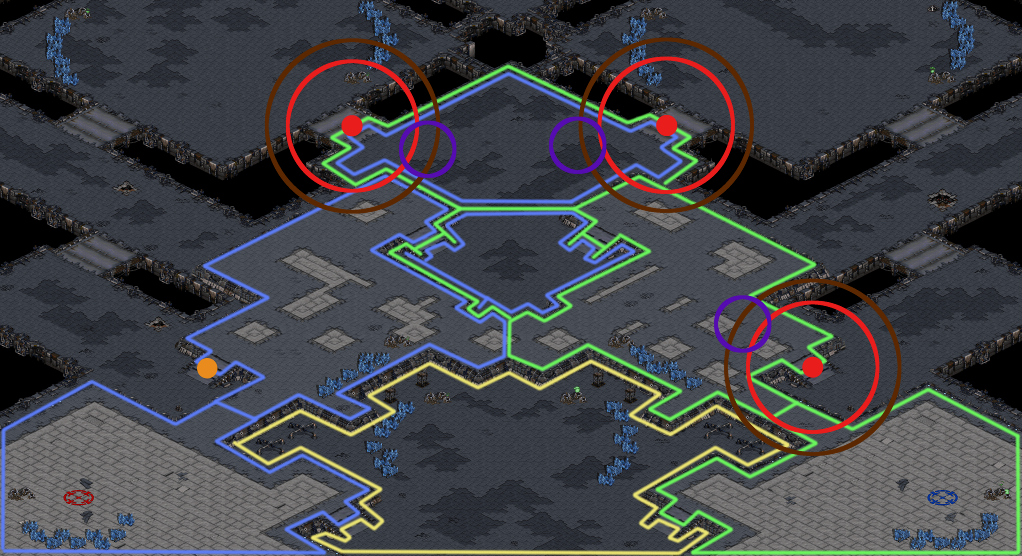
\includegraphics[width=\textwidth]{space_atoll_(co-op)_defense_locations}
\caption{Example of defense locations. \colorbox{LightGreen}{BATS’s regions}, \colorbox{LightBlue}{allied’s regions}, regions outlined with both green and blue belong to \fcolorbox{LightBlue}{LightGreen}{both}. \colorbox{Yellow}{Non-defended} as they abut only BATS or allied regions. \colorbox{Red}{Defense locations} are both the dot and the smallest circle is the \colorbox{Red}{defend perimeter} whereas the outer circle is the \colorbox{Brown}{\textcolor{white}{enemy offensive perimeter}}. The orange dot is the \colorbox{Orange}{teammate's defense location}.}
\label{fig:defense_locations}
\end{figure}

Patrol squads on the other hand contains all free units, these will patrol between the defense locations. If enemy units enter the enemy offensive perimeter (\squadDefendEnemyOffensivePerimeter~in radius) in a defense location all squad units will move to the defend location to defend it, all other hold squads will disband to join the defense in the patrol squad. The idea was first to only disband the other hold squads if the enemy is too strong, but the calculation proved difficult and we focused work on other more improtant areas. This strategy was tested and it works good against one StarCraft default AI, as it only attacks from one location at a time. Two default AIs can however attack from different locations, but usually attacked from one location, but was in general too strong for BATS to defend by itself. Although it worked against the default AI it would not work against other AIs or humans that can attack two different locations simultaneously.


Both hold squads and patrol squads roam or patrol between BATS’s defense location so the bot won’t disturb the allied player with its units.

\paragraph{Defending other locations}
Although no hold squads are located on and the patrol squad never patrols on the teammates defend locations. It will still send the patrol squad to defend a teammate defend locations if BATS is not under attack itself. In addition to defending all defend locations, the defense manager will send out the patrol squad to defend locations either inside BATS’s or the teammate's base that are under attack, for example if the enemy drops inside the base. This will, however, never bring the hold squads as they should defend the entrance to the base.